% !TEX program = xelatex
\documentclass[12pt,a4paper]{report}

% --- Cấu hình Tiếng Việt và Font cho Overleaf (XeLaTeX) ---
\usepackage{fontspec}
\usepackage[vietnamese]{babel}
\usepackage{amsmath, amssymb, amsfonts}
\usepackage{graphicx}
\usepackage{hyperref}
\usepackage{titlesec}
\usepackage{booktabs} 
\usepackage{geometry}
\usepackage{enumitem} % Tùy chỉnh danh sách
\geometry{a4paper, margin=2.5cm}

% Sử dụng font Times New Roman chuẩn học thuật
\setmainfont{Times New Roman}

% Cấu hình tiêu đề chương và phần
\titleformat{\chapter}[display]
  {\normalfont\huge\bfseries}{\chaptername\ \thechapter}{20pt}{\Huge}
\titlespacing*{\chapter}{0pt}{-20pt}{40pt}

\begin{document}

\chapter{Từ Monolithic đến Microservice và DDD}

\section{Kiến trúc đơn khối (Monolithic Architecture)}
\subsection{Khái niệm và Bản chất Kỹ thuật}
Kiến trúc Monolithic không chỉ đơn thuần là việc đóng gói mã nguồn vào một tệp tin thực thi (như .war hay .jar), mà còn đại diện cho một tư duy thiết kế tập trung. Trong mô hình này, toàn bộ logic nghiệp vụ, giao diện người dùng, và các thành phần truy xuất dữ liệu được liên kết chặt chẽ (tightly coupled) trong một đơn vị duy nhất. 

Sự gắn kết này có nghĩa là các thành phần chia sẻ chung bộ nhớ, tài nguyên CPU và thường là một cơ sở dữ liệu quan hệ duy nhất. Bất kỳ thay đổi nhỏ nào trong một module cũng đòi hỏi việc biên dịch lại và triển khai lại toàn bộ hệ thống.

\subsection{Cấu trúc Phân lớp điển hình}
Đa số các hệ thống Monolithic hiện đại được tổ chức theo mô hình **Layered Architecture** (Kiến trúc phân lớp):
\begin{itemize}
    \item \textbf{Presentation Layer:} Xử lý giao diện người dùng và các yêu cầu HTTP.
    \item \textbf{Business Logic Layer:} Chứa các quy tắc nghiệp vụ cốt lõi của hệ thống.
    \item \textbf{Data Access Layer (DAL):} Chịu trách nhiệm giao tiếp với cơ sở dữ liệu.
\end{itemize}

Mặc dù được phân lớp về mặt logic, nhưng ở cấp độ vật lý, chúng vẫn chạy chung một tiến trình (process).

\subsection{Ưu điểm và Hạn chế trong Vận hành}
\textbf{Ưu điểm:}
\begin{itemize}
    \item \textbf{Đơn giản trong quản lý:} Quá trình kiểm thử tích hợp (End-to-End testing) diễn ra thuận lợi do không có độ trễ mạng giữa các thành phần.
    \item \textbf{Hiệu suất tối ưu:} Các lời gọi hàm trực tiếp trong bộ nhớ luôn nhanh hơn việc gọi qua API hoặc Message Broker.
    \item \textbf{Nhất quán dữ liệu (ACID):} Việc sử dụng một DB duy nhất giúp đảm bảo tính toàn vẹn dữ liệu thông qua các Transaction truyền thống.
\end{itemize}

\textbf{Hạn chế (The Big Ball of Mud):}
\begin{itemize}
    \item \textbf{Rào cản về quy mô (Scalability):} Không thể mở rộng riêng biệt một module bị nghẽn (ví dụ: module xử lý thanh toán), buộc phải nhân bản toàn bộ ứng dụng, gây lãng phí tài nguyên.
    \item \textbf{Sự trì trệ về công nghệ (Technology Lock-in):} Việc nâng cấp một thư viện hoặc ngôn ngữ mới là cực kỳ rủi ro vì nó ảnh hưởng đến tất cả các phần còn lại.
\end{itemize}

\section{Kiến trúc Dịch vụ nhỏ (Microservices Architecture)}
\subsection{Triết lý thiết kế và Đặc điểm cốt lõi}
Khác với Monolithic, Microservices tuân thủ triết lý "Làm một việc và làm thật tốt" (Do one thing and do it well). Mỗi dịch vụ là một thực thể độc lập, có vòng đời phát triển và triển khai riêng biệt. 

Đặc điểm quan trọng nhất là **Bao đóng dữ liệu (Data Encapsulation)**: Mỗi microservice sở hữu cơ sở dữ liệu riêng (Database per Service), ngăn chặn việc truy cập dữ liệu trực tiếp từ các dịch vụ khác, từ đó giảm thiểu sự phụ thuộc.

\subsection{Hệ sinh thái và Các thành phần bổ trợ}
Để một hệ thống Microservices vận hành ổn định, cần có các thành phần hạ tầng phức tạp:
\begin{itemize}
    \item \textbf{API Gateway:} Điểm tiếp nhận duy nhất cho client, chịu trách nhiệm định tuyến, xác thực và giới hạn lưu lượng.
    \item \textbf{Service Discovery:} Cho phép các dịch vụ tìm thấy nhau trong môi trường mạng động (ví dụ: Netflix Eureka, Consul).
    \item \textbf{Circuit Breaker:} Cơ chế ngăn chặn lỗi dây chuyền khi một dịch vụ gặp sự cố (ví dụ: Hystrix hoặc Resilience4j).
\end{itemize}


\subsection{Thách thức về Quản trị và Nhất quán dữ liệu}
Mặc dù mang lại sự linh hoạt, Microservices đối mặt với bài toán **Nhất quán sau cùng (Eventual Consistency)**. Do dữ liệu bị phân tán, việc thực hiện các giao dịch phân tán (Distributed Transactions) trở nên cực kỳ khó khăn, thường phải áp dụng các mô hình như **Saga Pattern** để điều phối.

\section{Phân tích so sánh: Khi nào nên chuyển đổi?}
Việc lựa chọn kiến trúc không dựa trên xu hướng, mà dựa trên "Complexity-Value Curve" (Đường cong giá trị và độ phức tạp). 
\begin{itemize}
    \item Với các dự án khởi nghiệp cần MVP nhanh, Monolithic là sự lựa chọn tối ưu. 
    \item Khi số lượng lập trình viên tăng lên (trên 20-30 người) và các yêu cầu nghiệp vụ trở nên quá chồng chéo, việc phân rã sang Microservices trở thành yếu tố sống còn để duy trì tốc độ phát triển.
\end{itemize}

\section{Thiết kế hướng tên miền (Domain-Driven Design - DDD)}
\subsection{Tại sao DDD là chìa khóa cho Microservices?}
Một trong những lỗi lớn nhất khi triển khai Microservices là phân rã dịch vụ theo kỹ thuật (ví dụ: Service DB, Service UI). DDD giải quyết vấn đề này bằng cách tập trung vào nghiệp vụ cốt lõi.

\subsection{Chiến lược thiết kế (Strategic Design)}
Khái niệm quan trọng nhất là **Bounded Context** (Ngữ cảnh bao đóng). Nó xác định ranh giới logic mà trong đó một mô hình dữ liệu có ý nghĩa nhất định. Ví dụ: Từ "Sản phẩm" trong ngữ cảnh "Bán hàng" sẽ khác with "Sản phẩm" trong ngữ cảnh "Kho bãi". Việc xác định đúng các Bounded Context chính là bước đầu tiên để xác định ranh giới của các Microservices.

\subsection{Context Mapping: Bản đồ tương tác}
Context Map giúp mô tả mối quan hệ giữa các ngữ cảnh:
\begin{itemize}
    \item \textbf{Shared Kernel:} Hai ngữ cảnh chia sẻ chung một phần mô hình.
    \item \textbf{Anticorruption Layer (ACL):} Lớp đệm giúp dịch vụ mới không bị ảnh hưởng bởi thiết kế lỗi thời của hệ thống cũ.
\end{itemize}

\subsection{Thiết kế kỹ thuật (Tactical Design)}
Để thực thi logic bên trong một Microservice, DDD cung cấp các công cụ:
\begin{itemize}
    \item \textbf{Aggregate:} Một cụm các đối tượng dữ liệu được coi là một đơn vị để thay đổi dữ liệu.
    \item \textbf{Value Objects:} Các đối tượng không có định danh, chỉ chứa giá trị (như Địa chỉ, Tiền tệ).
    \item \textbf{Repositories:} Lớp trung gian giữa Domain và Data Mapping.
\end{itemize}

\chapter{Phát triển Hệ thống E-Commerce dựa trên Microservices}

\section{Xác định yêu cầu hệ thống}
Trong bối cảnh thị trường thương mại điện tử cạnh tranh khốc liệt, việc xây dựng một hệ thống có khả năng thích ứng nhanh và quy mô lớn là điều bắt buộc. Hệ thống được thiết kế để phục vụ cả khách hàng (Customer) và nhân viên quản trị (Staff), tích hợp trí tuệ nhân tạo (AI) để tối ưu hóa trải nghiệm người dùng.

\subsection{Yêu cầu chức năng (Functional Requirements)}
Hệ thống bao gồm các nhóm chức năng chính sau:
\begin{itemize}
    \item \textbf{Quản lý người dùng và xác thực:} Cho phép khách hàng đăng ký, đăng nhập và quản lý thông tin cá nhân. Nhân viên có các quyền hạn riêng biệt theo vai trò (Role-based Access Control).
    \item \textbf{Quản lý danh mục sản phẩm:} Hiển thị và quản lý thông tin chi tiết các dòng Laptop và Mobile, bao gồm cấu hình kỹ thuật, giá cả và chương trình khuyến mãi.
    \item \textbf{Hệ thống giỏ hàng:} Cho phép người dùng thêm, bớt sản phẩm từ các dịch vụ khác nhau (Laptop/Mobile) vào một giỏ hàng nhất nhất quán.
    \item \textbf{Tư vấn thông minh (AI Chatbot):} Cung cấp khả năng trả lời tự động các thắc mắc về sản phẩm dựa trên cơ sở tri thức (Knowledge Base) được trích xuất từ cơ sở dữ liệu đồ thị.
\end{itemize}

\subsection{Yêu cầu phi chức năng (Non-functional Requirements)}
Để đảm bảo chất lượng dịch vụ cấp doanh nghiệp, hệ thống cần đáp ứng:
\begin{itemize}
    \item \textbf{Tính mở rộng (Scalability):} Khả năng mở rộng độc lập các dịch vụ có tải cao như Laptop Service hoặc AI Service mà không ảnh hưởng đến toàn bộ hệ thống.
    \item \textbf{Tính sẵn sàng cao (High Availability):} Hệ thống phải hoạt động liên tục, giảm thiểu điểm chết duy nhất (Single Point of Failure) thông qua cơ chế replication và load balancing.
    \item \textbf{Tính bảo mật (Security):} Dữ liệu người dùng phải được mã hóa, các API được bảo vệ qua Gateway và cơ chế xác thực tập trung.
    \item \textbf{Khả năng bảo trì (Maintainability):} Mã nguồn được tổ chức theo cấu trúc chuẩn của Django và Microservices, giúp dễ dàng nâng cấp và sửa lỗi từng phần.
\end{itemize}

\section{Phân rã hệ thống theo thiết kế hướng tên miền (DDD)}
Việc phân rã hệ thống dựa trên nghiệp vụ thay vì kỹ thuật giúp đảm bảo tính bao đóng và giảm thiểu sự phụ thuộc chồng chéo.

\subsection{Xác định các Ngữ cảnh bao đóng (Bounded Contexts)}
Dựa trên phân tích nghiệp vụ, hệ thống được chia thành 5 Bounded Contexts chính:
\begin{itemize}
    \item \textbf{Customer Context:} Tập trung vào thực thể khách hàng và quy trình tương tác của họ với hệ thống (Login, Register, Cart).
    \item \textbf{Laptop Context:} Quản lý chuyên sâu về các sản phẩm máy tính xách tay với các đặc tính kỹ thuật riêng biệt (CPU, GPU, Screen).
    \item \textbf{Mobile Context:} Quản lý các thiết bị di động với các thuộc tính như Camera, dung lượng Pin.
    \item \textbf{Staff Context:} Quản lý nhân sự và các hoạt động quản trị nội bộ.
    \item \textbf{AI Context:} Cung cấp các khả năng thông minh, xử lý ngôn ngữ tự nhiên để tư vấn bán hàng.
\end{itemize}

\subsection{Các nguyên tắc và ràng buộc kiến trúc}
Hệ thống tuân thủ các ràng buộc nghiêm ngặt:
\begin{itemize}
    \item \textbf{Database per Service:} Mỗi ngữ cảnh sở hữu một cơ sở dữ liệu riêng, đảm bảo tính cô lập hoàn toàn về dữ liệu.
    \item \textbf{Polyglot Persistence:} Sử dụng đa dạng các loại cơ sở dữ liệu (PostgreSQL cho dữ liệu quan hệ và Neo4j cho dữ liệu đồ thị phục vụ AI).
    \item \textbf{Giao tiếp qua API/Gateway:} Các dịch vụ không gọi trực tiếp cơ sở dữ liệu của nhau mà phải thông qua các giao diện lập trình ứng dụng (API).
\end{itemize}

\section{Thiết kế và Triển khai Customer Service}
Customer Service đóng vai trò là điểm chạm đầu tiên của người dùng, xử lý các nghiệp vụ liên quan đến định danh và quản lý trạng thái mua hàng.

\subsection{Logic nghiệp vụ}
\begin{itemize}
    \item \textbf{Quản lý danh tính:} Xử lý quy trình đăng ký tài khoản mới và xác thực người dùng dựa trên thông tin định danh duy nhất.
    \item \textbf{Quản lý giỏ hàng tập trung:} Khởi tạo giỏ hàng riêng biệt cho mỗi khách hàng ngay khi đăng ký.
    \item \textbf{Xử lý vật phẩm đa dạng:} Cho phép thêm các loại sản phẩm khác nhau (Laptop, Mobile) vào chung một giỏ hàng bằng cách lưu trữ mã định danh và loại sản phẩm.
    \item \textbf{Cập nhật số lượng thông minh:} Tự động kiểm tra sự tồn tại của vật phẩm trong giỏ; nếu đã tồn tại, hệ thống sẽ cộng dồn số lượng thay vì tạo bản ghi mới.
\end{itemize}

\subsection{Mô hình dữ liệu (Data Models)}
Hệ thống sử dụng các thực thể chính sau:
\begin{itemize}
    \item \textbf{Customer:}
        \begin{itemize}
            \item \texttt{name}: Họ và tên khách hàng (String).
            \item \texttt{phone}: Số điện thoại liên lạc (String).
            \item \texttt{email}: Địa chỉ thư điện tử (Unique Email).
            \item \texttt{username}: Tên đăng nhập (Unique String).
            \item \texttt{password}: Mật khẩu đã được băm (Hash String).
        \end{itemize}
    \item \textbf{Cart:}
        \begin{itemize}
            \item \texttt{customer}: Liên kết 1-1 với thực thể Customer.
        \end{itemize}
    \item \textbf{CartItem:}
        \begin{itemize}
            \item \texttt{item\_id}: ID của sản phẩm từ dịch vụ ngoại lai (Integer).
            \item \texttt{product\_type}: Loại sản phẩm (MOBILE hoặc LAPTOP).
            \item \texttt{quantity}: Số lượng sản phẩm trong giỏ (Positive Integer).
            \item \texttt{cart}: Liên kết N-1 với thực thể Cart.
        \end{itemize}
\end{itemize}

\begin{figure}[h!]
    \centering
    \includegraphics[width=0.8\textwidth]{"Class Diagram.png"}
    \caption{Sơ đồ lớp (Class Diagram)}
    \label{fig:class-diagram}
\end{figure}

\subsection{Thiết kế CSDL}
\begin{figure}[h!]
    \centering
    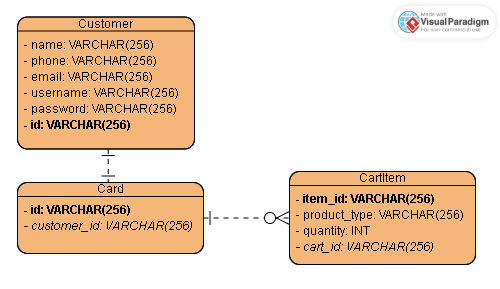
\includegraphics[width=0.8\textwidth]{Customer_DB.png}
    \caption{Thiết kế Cơ sở dữ liệu Customer Service}
    \label{fig:customer-db}
\end{figure}

\subsection{Xây dựng cơ sở dữ liệu}
\textbf{Cơ sở dữ liệu sử dụng:} MySQL.

\textbf{Lý do lựa chọn:} MySQL là hệ quản trị cơ sở dữ liệu quan hệ (RDBMS) phổ biến, mã nguồn mở, có hiệu suất cao cho các tác vụ đọc/ghi thông tin người dùng và giỏ hàng. Nó đảm bảo tính nhất quán dữ liệu (ACID) cần thiết cho các giao dịch liên quan đến khách hàng.

\textbf{Mã nguồn định nghĩa các bảng (Django Models):}
\begin{verbatim}
class Customer(models.Model):
    name = models.CharField(max_length=255)
    phone = models.CharField(max_length=20)
    email = models.EmailField(unique=True)
    username = models.CharField(max_length=150, unique=True)
    password = models.CharField(max_length=255)

class Cart(models.Model):
    customer = models.OneToOneField(Customer, on_delete=models.CASCADE)

class CartItem(models.Model):
    item_id = models.IntegerField()
    cart = models.ForeignKey(Cart, on_delete=models.CASCADE)
    quantity = models.PositiveIntegerField(default=1)
    product_type = models.CharField(max_length=10, 
                                   choices=(('MOBILE', 'MOBILE'), ('LAPTOP', 'LAPTOP')))
\end{verbatim}

\textbf{Phương pháp Seed dữ liệu:}
Hệ thống sử dụng Django Management Command để khởi tạo dữ liệu mẫu. Lệnh thực hiện:
\begin{verbatim}
python manage.py seed_db
\end{verbatim}
Dữ liệu được tạo bao gồm các tài khoản khách hàng mặc định và giỏ hàng trống tương ứng để sẵn sàng cho việc mua sắm.

\subsection{Giao diện lập trình ứng dụng (API Endpoints)}
\begin{table}[h!]
\centering
\begin{tabular}{|l|c|p{4cm}|p{3cm}|p{3cm}|}
\hline
\textbf{Endpoint} & \textbf{Method} & \textbf{Tác dụng} & \textbf{Dữ liệu yêu cầu} & \textbf{Dữ liệu trả về} \\ \hline
\texttt{/register/} & POST & Đăng ký tài khoản & Thông tin Customer & JSON khách hàng \\ \hline
\texttt{/login/} & POST & Xác thực người dùng & Username, Password & Thông tin khách hàng \\ \hline
\texttt{/cart-items/} & GET & Liệt kê vật phẩm & Token xác thực & List CartItems \\ \hline
\texttt{/cart-items/} & POST & Thêm vào giỏ & \texttt{item\_id, type, qty} & CartItem chi tiết \\ \hline
\end{tabular}
\end{table}

\section{Thiết kế và Triển khai Laptop Service}
Dịch vụ quản lý kho dữ liệu và đặc tính kỹ thuật của các dòng máy tính xách tay.

\subsection{Logic nghiệp vụ}
\begin{itemize}
    \item \textbf{Phân loại sản phẩm:} Tổ chức máy tính theo hãng sản xuất và danh mục sử dụng (Gaming, Văn phòng, v.v.).
    \item \textbf{Quản lý cấu hình chi tiết:} Lưu trữ các thông số phần cứng chuyên sâu phục vụ việc so sánh và tra cứu.
    \item \textbf{Đồng bộ hóa dữ liệu đồ thị:} Cung cấp dữ liệu để ánh xạ sang Neo4j, xây dựng mạng lưới liên kết giữa sản phẩm và các thành phần phần cứng.
\end{itemize}

\subsection{Mô hình dữ liệu (Data Models)}
\begin{itemize}
    \item \textbf{Mô hình quan hệ (Relational Model):}
        \begin{itemize}
            \item \textbf{Laptop:} \texttt{name, img\_url, price, discount, ram, cpu, gpu, screen}.
            \item \textbf{Manufacturer / Category}: Chỉ bao gồm trường \texttt{name} để định danh.
        \end{itemize}
    \item \textbf{Mô hình đồ thị (Graph Model):}
        \begin{itemize}
            \item \textbf{Nodes:} \texttt{Laptop, CPU, GPU, RAM, Screen, Manufacturer}.
            \item \textbf{Relationships:} \texttt{HAS\_CPU, MADE\_BY, BELONGS\_TO}.
        \end{itemize}
\end{itemize}

\subsection{Thiết kế CSDL}
\begin{figure}[h!]
    \centering
    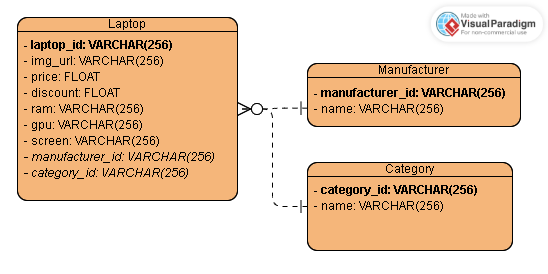
\includegraphics[width=0.8\textwidth]{Laptop_DB.png}
    \caption{Thiết kế Cơ sở dữ liệu Laptop Service}
    \label{fig:laptop-db}
\end{figure}

\subsection{Xây dựng cơ sở dữ liệu}
\textbf{Cơ sở dữ liệu sử dụng:} PostgreSQL (Relational) và Neo4j (Graph).

\textbf{Lý do lựa chọn:} 
\begin{itemize}
    \item \textbf{PostgreSQL:} Được sử dụng để lưu trữ dữ liệu sản phẩm có cấu trúc chặt chẽ. PostgreSQL hỗ trợ tốt các kiểu dữ liệu phức tạp và khả năng mở rộng mạnh mẽ cho danh mục sản phẩm lớn.
    \item \textbf{Neo4j:} Được sử dụng để lưu trữ các mối quan hệ kỹ thuật giữa Laptop và phần cứng (CPU, GPU, RAM). Điều này cho phép AI Service truy vấn và so sánh cấu hình một cách nhanh chóng thông qua các thuật toán đồ thị.
\end{itemize}

\textbf{Mã nguồn định nghĩa các bảng (Django Models):}
\begin{verbatim}
class Manufacturer(models.Model):
    name = models.CharField(max_length=255)

class Category(models.Model):
    name = models.CharField(max_length=255)

class Laptop(models.Model):
    name = models.CharField(max_length=255)
    img_url = models.URLField(max_length=500)
    price = models.DecimalField(max_digits=12, decimal_places=2)
    manufacturer = models.ForeignKey(Manufacturer, on_delete=models.CASCADE)
    category = models.ForeignKey(Category, on_delete=models.CASCADE)
    ram = models.CharField(max_length=50)
    cpu = models.CharField(max_length=255)
    gpu = models.CharField(max_length=255)
    screen = models.CharField(max_length=255)
\end{verbatim}

\textbf{Phương pháp Seed dữ liệu:}
Dữ liệu được khởi tạo thông qua script Python độc lập. Lệnh thực hiện:
\begin{verbatim}
python seed_db.py
\end{verbatim}
Script này sẽ tự động tạo các bản ghi cho Hãng sản xuất, Danh mục và danh sách các Laptop mẫu cùng thông số kỹ thuật chi tiết.

\subsection{Giao diện lập trình ứng dụng (API Endpoints)}
\begin{table}[h!]
\centering
\begin{tabular}{|l|c|p{4cm}|p{3cm}|p{3cm}|}
\hline
\textbf{Endpoint} & \textbf{Method} & \textbf{Tác dụng} & \textbf{Dữ liệu yêu cầu} & \textbf{Dữ liệu trả về} \\ \hline
\texttt{/laptops/} & GET & Lấy danh sách sản phẩm & Tham số lọc (tùy chọn) & Danh sách Laptop \\ \hline
\texttt{/laptops/\{id\}/} & GET & Chi tiết sản phẩm & ID sản phẩm & Đối tượng Laptop \\ \hline
\texttt{/manufacturers/} & GET & Lấy danh sách hãng & Không & Danh sách hãng \\ \hline
\end{tabular}
\end{table}

\section{Thiết kế và Triển khai Mobile Service}
Quản lý dải sản phẩm thiết bị di động và các đặc thù công nghệ liên quan.

\subsection{Logic nghiệp vụ}
\begin{itemize}
    \item \textbf{Quản lý thông số di động:} Tập trung vào các yếu tố người dùng quan tâm như Camera và hiệu năng xử lý.
    \item \textbf{Phân mảnh thị trường:} Hỗ trợ phân loại sản phẩm theo thương hiệu để người dùng dễ dàng tiếp cận.
\end{itemize}

\subsection{Mô hình dữ liệu (Data Models)}
\begin{itemize}
    \item \textbf{Mobile:}
        \begin{itemize}
            \item \texttt{name, price, discount, camera}: Thuộc tính cơ bản và đặc thù.
            \item \texttt{ram, cpu, gpu}: Cấu hình hiệu năng.
            \item \texttt{manufacturer, category}: Tham chiếu thực thể cha.
        \end{itemize}
\end{itemize}

\subsection{Thiết kế CSDL}
\begin{figure}[h!]
    \centering
    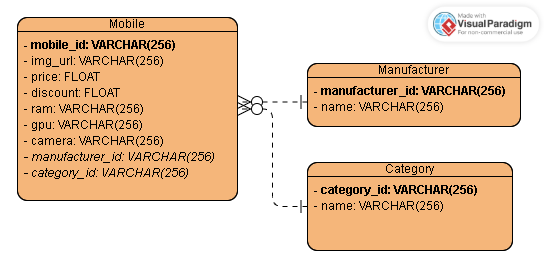
\includegraphics[width=0.8\textwidth]{Mobile_DB.png}
    \caption{Thiết kế Cơ sở dữ liệu Mobile Service}
    \label{fig:mobile-db}
\end{figure}

\subsection{Xây dựng cơ sở dữ liệu}
\textbf{Cơ sở dữ liệu sử dụng:} PostgreSQL và Neo4j.

\textbf{Lý do lựa chọn:} Tương tự như Laptop Service, Mobile Service sử dụng PostgreSQL cho các thuộc tính thương mại và Neo4j cho các mối quan hệ kỹ thuật. Sự kết hợp này giúp hệ thống vừa đảm bảo tính nhất quán giao dịch, vừa tối ưu cho các tính năng thông minh của AI Chatbot khi cần so sánh các thông số như Camera hay dung lượng Pin giữa các dòng điện thoại.

\textbf{Mã nguồn định nghĩa các bảng (Django Models):}
\begin{verbatim}
class Manufacturer(models.Model):
    name = models.CharField(max_length=255)

class Category(models.Model):
    name = models.CharField(max_length=255)

class Mobile(models.Model):
    name = models.CharField(max_length=255)
    img_url = models.URLField(max_length=500)
    price = models.DecimalField(max_digits=12, decimal_places=2)
    manufacturer = models.ForeignKey(Manufacturer, on_delete=models.CASCADE)
    category = models.ForeignKey(Category, on_delete=models.CASCADE)
    ram = models.CharField(max_length=50)
    cpu = models.CharField(max_length=255)
    gpu = models.CharField(max_length=255)
    camera = models.CharField(max_length=255)
\end{verbatim}

\textbf{Phương pháp Seed dữ liệu:}
Sử dụng Django Management Command để khởi tạo danh mục điện thoại. Lệnh thực hiện:
\begin{verbatim}
python manage.py seed_db
\end{verbatim}
Dữ liệu mẫu bao gồm các dòng Flagship phổ biến như iPhone, Samsung Galaxy, Xiaomi,... cùng các thông số phần cứng tương ứng.

\subsection{Giao diện lập trình ứng dụng (API Endpoints)}
\begin{table}[h!]
\centering
\begin{tabular}{|l|c|p{4cm}|p{3cm}|p{3cm}|}
\hline
\textbf{Endpoint} & \textbf{Method} & \textbf{Tác dụng} & \textbf{Dữ liệu yêu cầu} & \textbf{Dữ liệu trả về} \\ \hline
\texttt{/mobiles/} & GET & Danh sách điện thoại & Không & List Mobile \\ \hline
\texttt{/mobiles/\{id\}/} & GET & Xem chi tiết & ID & Chi tiết Mobile \\ \hline
\end{tabular}
\end{table}

\section{Thiết kế và Triển khai Staff Service}
Hệ thống quản trị dành cho nhân sự vận hành sàn thương mại điện tử.

\subsection{Logic nghiệp vụ}
\begin{itemize}
    \item \textbf{Kiểm soát truy cập (RBAC):} Phân quyền nhân viên theo các vai trò khác nhau trong hệ thống.
    \item \textbf{Quản lý vận hành:} Cung cấp giao diện để nhân viên theo dõi trạng thái hệ thống và dữ liệu sản phẩm.
\end{itemize}

\subsection{Mô hình dữ liệu (Data Models)}
\begin{itemize}
    \item \textbf{Staff:}
        \begin{itemize}
            \item \texttt{staff\_id}: Mã nhân viên duy nhất.
            \item \texttt{name, phone, email}: Thông tin liên lạc cá nhân.
            \item \texttt{username, password}: Thông tin đăng nhập.
            \item \texttt{role}: Vai trò (Admin, Manager, v.v.).
        \end{itemize}
\end{itemize}

\subsection{Thiết kế CSDL}
\begin{figure}[h!]
    \centering
    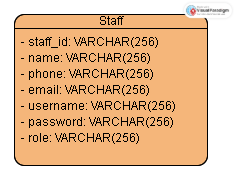
\includegraphics[width=0.8\textwidth]{Staff_DB.png}
    \caption{Thiết kế Cơ sở dữ liệu Staff Service}
    \label{fig:staff-db}
\end{figure}

\subsection{Xây dựng cơ sở dữ liệu}
\textbf{Cơ sở dữ liệu sử dụng:} MySQL.

\textbf{Lý do lựa chọn:} MySQL cung cấp cơ chế bảo mật và quản lý người dùng mạnh mẽ, phù hợp để lưu trữ thông tin nhân sự và quyền hạn truy cập hệ thống. Tính ổn định và khả năng xử lý đồng thời của MySQL giúp nhân viên thực hiện các thao tác quản trị một cách mượt mà.

\textbf{Mã nguồn định nghĩa các bảng (Django Models):}
\begin{verbatim}
class Staff(models.Model):
    staff_id = models.CharField(max_length=50, unique=True)
    name = models.CharField(max_length=255)
    phone = models.CharField(max_length=20)
    email = models.EmailField(unique=True)
    username = models.CharField(max_length=150, unique=True)
    password = models.CharField(max_length=255)
    role = models.CharField(max_length=100)
\end{verbatim}

\textbf{Phương pháp Seed dữ liệu:}
Lệnh thực hiện:
\begin{verbatim}
python manage.py seed_db
\end{verbatim}
Dữ liệu khởi tạo bao gồm tài khoản Quản trị hệ thống (System Administrator) và các nhân viên mẫu với các vai trò khác nhau (Admin, Manager, Staff) để phục vụ việc kiểm thử phân quyền.

\subsection{Giao diện lập trình ứng dụng (API Endpoints)}
\begin{table}[h!]
\centering
\begin{tabular}{|l|c|p{4cm}|p{3cm}|p{3cm}|}
\hline
\textbf{Endpoint} & \textbf{Method} & \textbf{Tác dụng} & \textbf{Dữ liệu yêu cầu} & \textbf{Dữ liệu trả về} \\ \hline
\texttt{/login/} & POST & Đăng nhập quản trị & Credentials & Staff Profile \\ \hline
\end{tabular}
\end{table}

\chapter{AI Service}

\section{Mục đích của AI Service}
AI Service trong hệ thống được xây dựng nhằm mục đích tối ưu hóa quy trình tư vấn khách hàng. Thay vì nhân viên phải trực tiếp trả lời các thắc mắc lặp đi lặp lại về thông số kỹ thuật, AI Service đóng vai trò là một trợ lý ảo thông minh:
\begin{itemize}
    \item \textbf{Tư vấn 24/7:} Phản hồi khách hàng ngay lập tức tại mọi thời điểm.
    \item \textbf{Độ chính xác cao:} Cung cấp thông tin dựa trên dữ liệu thực tế được trích xuất từ kho hàng.
    \item \textbf{Cá nhân hóa trải nghiệm:} Hiểu ý định người dùng để đưa ra các gợi ý sản phẩm phù hợp.
\end{itemize}

\section{Kiến trúc tổng quan AI Service}
Dịch vụ được xây dựng trên nền tảng Django REST Framework, tích hợp trực tiếp các thư viện học máy hiện đại:
\begin{itemize}
    \item \textbf{Hugging Face Transformers:} Thư viện lõi để triển khai và chạy mô hình ngôn ngữ lớn (LLM).
    \item \textbf{Neomodel:} Thư viện Object-Graph Mapping (OGM) để giao tiếp với cơ sở dữ liệu đồ thị Neo4j.
    \item \textbf{PyTorch:} Backend tính toán cho mô hình AI.
    \item \textbf{Background Loading:} Mô hình AI được tải trong một tiến trình chạy ngầm (threading) để không làm gián đoạn quá trình khởi động của server.
\end{itemize}

\section{Logic hoạt động của Chatbot}
Quy trình xử lý một yêu cầu của chatbot diễn ra theo các bước sau:
\begin{enumerate}
    \item \textbf{Tiếp nhận:} API nhận \texttt{user\_message} từ client qua phương thức POST.
    \item \textbf{Trích xuất tri thức:} Hệ thống gọi hàm \texttt{get\_knowledge\_base()} để lấy toàn bộ thông tin sản phẩm (Laptop và Mobile) từ Neo4j.
    \item \textbf{Xây dựng ngữ cảnh (Context):} Dữ liệu thô từ database được định dạng thành văn bản liệt kê tên sản phẩm, giá và cấu hình.
    \item \textbf{Tạo Prompt:} Kết hợp ngữ cảnh sản phẩm và câu hỏi của người dùng vào một cấu trúc template quy định vai trò của trợ lý.
    \item \textbf{Suy luận (Inference):} Mô hình AI xử lý prompt và sinh câu trả lời.
    \item \textbf{Phản hồi:} Câu trả lời được tách khỏi định dạng prompt và gửi về cho người dùng.
\end{enumerate}

\section{Kiến trúc Mô hình AI sử dụng}
\textbf{Mô hình:} TinyLlama/TinyLlama-1.1B-Chat-v1.0.

\textbf{Cấu hình kỹ thuật:}
\begin{itemize}
    \item \textbf{Device:} Chạy trên CPU thay vì GPU.
    \item \textbf{Dtype:} \texttt{torch.float32} để đảm bảo tính tương thích và chính xác trên CPU.
    \item \textbf{Max New Tokens:} 64 tokens (giới hạn độ dài câu trả lời để tăng tốc độ phản hồi).
    \item \textbf{Decoding Strategy:} \texttt{do\_sample=False} (sử dụng Greedy Search để câu trả lời mang tính nhất quán và ổn định nhất).
\end{itemize}

\textbf{Lý do lựa chọn và Đánh đổi:}
TinyLlama là mô hình nhỏ gọn với 1,1 tỷ tham số. Việc sử dụng mô hình này giúp hệ thống có thể chạy mượt mà trên môi trường containerized với tài nguyên CPU hạn chế mà không cần đến phần cứng chuyên dụng (GPU). Đánh đổi lại là khả năng lập luận phức tạp của mô hình sẽ hạn chế hơn so với các mô hình lớn (như Llama-2 70B), nhưng hoàn toàn đáp ứng tốt nhu cầu tư vấn thông số sản phẩm đơn giản.

\section{Knowledge Base và Neo4j}
\textbf{Cấu trúc tri thức:} AI Service sử dụng mô hình dữ liệu đồ thị để biểu diễn sản phẩm.
\begin{itemize}
    \item \textbf{Nodes:} Bao gồm các thực thể như \texttt{Laptop}, \texttt{Mobile}, \texttt{CPU}, \texttt{GPU}, \texttt{RAM}, \texttt{Manufacturer}.
    \item \textbf{Relationships:} Các mối quan hệ như \texttt{HAS\_CPU}, \texttt{MADE\_BY}, \texttt{HAS\_CAMERA} tạo thành một mạng lưới tri thức liên kết.
\end{itemize}

\textbf{Tại sao sử dụng Neo4j?}
Khác với SQL, Neo4j cho phép AI Service "nhìn" thấy các mối quan hệ giữa các linh kiện một cách trực tiếp. Điều này cực kỳ hữu ích khi chatbot cần thực hiện các truy vấn so sánh hoặc tìm kiếm sản phẩm có chung một đặc tính kỹ thuật cụ thể (ví dụ: "Tìm các laptop dùng chung CPU Intel Core i7").

\section{Kỹ thuật RAG (Retrieval-Augmented Generation)}
AI Service áp dụng kỹ thuật RAG đơn giản để khắc phục hiện tượng "ảo giác" (hallucination) của mô hình AI. Thay vì để mô hình tự nhớ thông số sản phẩm (vốn dễ sai lệch), hệ thống thực hiện:
\begin{itemize}
    \item \textbf{Retrieval:} Truy xuất thông tin thực tế từ Neo4j ngay tại thời điểm người dùng đặt câu hỏi.
    \item \textbf{Augmentation:} Bơm dữ liệu vừa truy xuất được vào \texttt{system\_prompt} dưới dạng "Tri thức nền tảng".
    \item \textbf{Generation:} Yêu cầu mô hình AI chỉ sinh câu trả lời dựa trên những thông tin đã cung cấp.
\end{itemize}
Cơ chế này đảm bảo chatbot không bao giờ tư vấn những sản phẩm không có trong kho hàng hoặc sai lệch về giá cả.

\section{Kiến trúc API Gateway và Điều phối}
Để che giấu sự phức tạp của hệ thống microservices phía sau, API Gateway được triển khai như một facade duy nhất. Nó chịu trách nhiệm proxy các yêu cầu đến đúng dịch vụ mục tiêu dựa trên đường dẫn URL, đồng thời xử lý các vấn đề xuyên suốt (cross-cutting concerns) như timeout và headers mapping.



\end{document}